\documentclass[a4paper, reqno, 12pt]{amsart}
% alternative choice:
%\documentclass[a4paper, reqno, 12pt]{article}
%\usepackage{authblk}    %comment this out when using amsart

\usepackage{amsthm,amsfonts,amssymb,amsmath,amsxtra,amsrefs}
\usepackage{xr-hyper}
\usepackage[colorlinks=
   citecolor=Black,
   linkcolor=Red,
   urlcolor=Blue]{hyperref}
\usepackage{verbatim}
\usepackage{tikz}
\usepackage[margin=1.25in]{geometry}
\usepackage{mathrsfs}
\usepackage{showkeys}

\newcommand{\remind}[1]{{\bf ** #1 **}}

\RequirePackage{xspace}
% load etoolbox package, for programming features
\RequirePackage{etoolbox}
% load varwidth package, for text environments which are automatically the natural width of the text they contain
\RequirePackage{varwidth}
% load enumitem package, for easy margin adjustment in enumerate and itemize environments
\RequirePackage{enumitem}
% load tensor package, for good placement of super/subscripts to the left of symbols
\RequirePackage{tensor}
% load mathtools package, for various extensions of amsmath
\RequirePackage{mathtools}
% load longtable package, which allows tables to (if needed) split over multiple pages
\RequirePackage{longtable}
% load multirow package, which allows cells spanning multiple rows in tables
\RequirePackage{multirow}



% put sections only (as opposed to subsections) in the table of contents
\setcounter{tocdepth}{1}


\def\ge{\geqslant}
\def\le{\leqslant}
\def\a{\alpha}
\def\b{\beta}
\def\g{\gamma}
\def\G{\Gamma}
\def\d{\delta}
\def\D{\Delta}
\def\L{\Lambda}
\def\e{\epsilon}
\def\et{\eta}
\def\io{\iota}
\def\o{\omega}
\def\p{\pi}
\def\ph{\phi}
\def\ps{\psi}
%\def\r{\rho}
\def\s{\sigma}
\def\t{\tau}
\def\th{\theta}
\def\k{\kappa}
\def\l{\lambda}
\def\z{\zeta}
\def\v{\vartheta}
\def\x{\xi}
\def\i{^{-1}}

\def\<{\langle}
\def\>{\rangle}

\newcommand{\sA}{\ensuremath{\mathscr{A}}\xspace}
\newcommand{\sB}{\ensuremath{\mathscr{B}}\xspace}
\newcommand{\sC}{\ensuremath{\mathscr{C}}\xspace}
\newcommand{\sD}{\ensuremath{\mathscr{D}}\xspace}
\newcommand{\sE}{\ensuremath{\mathscr{E}}\xspace}
\newcommand{\sF}{\ensuremath{\mathscr{F}}\xspace}
\newcommand{\sG}{\ensuremath{\mathscr{G}}\xspace}
\newcommand{\sH}{\ensuremath{\mathscr{H}}\xspace}
\newcommand{\sI}{\ensuremath{\mathscr{I}}\xspace}
\newcommand{\sJ}{\ensuremath{\mathscr{J}}\xspace}
\newcommand{\sK}{\ensuremath{\mathscr{K}}\xspace}
\newcommand{\sL}{\ensuremath{\mathscr{L}}\xspace}
\newcommand{\sM}{\ensuremath{\mathscr{M}}\xspace}
\newcommand{\sN}{\ensuremath{\mathscr{N}}\xspace}
\newcommand{\sO}{\ensuremath{\mathscr{O}}\xspace}
\newcommand{\sP}{\ensuremath{\mathscr{P}}\xspace}
\newcommand{\sQ}{\ensuremath{\mathscr{Q}}\xspace}
\newcommand{\sR}{\ensuremath{\mathscr{R}}\xspace}
\newcommand{\sS}{\ensuremath{\mathscr{S}}\xspace}
\newcommand{\sT}{\ensuremath{\mathscr{T}}\xspace}
\newcommand{\sU}{\ensuremath{\mathscr{U}}\xspace}
\newcommand{\sV}{\ensuremath{\mathscr{V}}\xspace}
\newcommand{\sW}{\ensuremath{\mathscr{W}}\xspace}
\newcommand{\sX}{\ensuremath{\mathscr{X}}\xspace}
\newcommand{\sY}{\ensuremath{\mathscr{Y}}\xspace}
\newcommand{\sZ}{\ensuremath{\mathscr{Z}}\xspace}


\newcommand{\fka}{\ensuremath{\mathfrak{a}}\xspace}
\newcommand{\fkb}{\ensuremath{\mathfrak{b}}\xspace}
\newcommand{\fkc}{\ensuremath{\mathfrak{c}}\xspace}
\newcommand{\fkd}{\ensuremath{\mathfrak{d}}\xspace}
\newcommand{\fke}{\ensuremath{\mathfrak{e}}\xspace}
\newcommand{\fkf}{\ensuremath{\mathfrak{f}}\xspace}
\newcommand{\fkg}{\ensuremath{\mathfrak{g}}\xspace}
\newcommand{\fkh}{\ensuremath{\mathfrak{h}}\xspace}
\newcommand{\fki}{\ensuremath{\mathfrak{i}}\xspace}
\newcommand{\fkj}{\ensuremath{\mathfrak{j}}\xspace}
\newcommand{\fkk}{\ensuremath{\mathfrak{k}}\xspace}
\newcommand{\fkl}{\ensuremath{\mathfrak{l}}\xspace}
\newcommand{\fkm}{\ensuremath{\mathfrak{m}}\xspace}
\newcommand{\fkn}{\ensuremath{\mathfrak{n}}\xspace}
\newcommand{\fko}{\ensuremath{\mathfrak{o}}\xspace}
\newcommand{\fkp}{\ensuremath{\mathfrak{p}}\xspace}
\newcommand{\fkq}{\ensuremath{\mathfrak{q}}\xspace}
\newcommand{\fkr}{\ensuremath{\mathfrak{r}}\xspace}
\newcommand{\fks}{\ensuremath{\mathfrak{s}}\xspace}
\newcommand{\fkt}{\ensuremath{\mathfrak{t}}\xspace}
\newcommand{\fku}{\ensuremath{\mathfrak{u}}\xspace}
\newcommand{\fkv}{\ensuremath{\mathfrak{v}}\xspace}
\newcommand{\fkw}{\ensuremath{\mathfrak{w}}\xspace}
\newcommand{\fkx}{\ensuremath{\mathfrak{x}}\xspace}
\newcommand{\fky}{\ensuremath{\mathfrak{y}}\xspace}
\newcommand{\fkz}{\ensuremath{\mathfrak{z}}\xspace}


\newcommand{\fkA}{\ensuremath{\mathfrak{A}}\xspace}
\newcommand{\fkB}{\ensuremath{\mathfrak{B}}\xspace}
\newcommand{\fkC}{\ensuremath{\mathfrak{C}}\xspace}
\newcommand{\fkD}{\ensuremath{\mathfrak{D}}\xspace}
\newcommand{\fkE}{\ensuremath{\mathfrak{E}}\xspace}
\newcommand{\fkF}{\ensuremath{\mathfrak{F}}\xspace}
\newcommand{\fkG}{\ensuremath{\mathfrak{G}}\xspace}
\newcommand{\fkH}{\ensuremath{\mathfrak{H}}\xspace}
\newcommand{\fkI}{\ensuremath{\mathfrak{I}}\xspace}
\newcommand{\fkJ}{\ensuremath{\mathfrak{J}}\xspace}
\newcommand{\fkK}{\ensuremath{\mathfrak{K}}\xspace}
\newcommand{\fkL}{\ensuremath{\mathfrak{L}}\xspace}
\newcommand{\fkM}{\ensuremath{\mathfrak{M}}\xspace}
\newcommand{\fkN}{\ensuremath{\mathfrak{N}}\xspace}
\newcommand{\fkO}{\ensuremath{\mathfrak{O}}\xspace}
\newcommand{\fkP}{\ensuremath{\mathfrak{P}}\xspace}
\newcommand{\fkQ}{\ensuremath{\mathfrak{Q}}\xspace}
\newcommand{\fkR}{\ensuremath{\mathfrak{R}}\xspace}
\newcommand{\fkS}{\ensuremath{\mathfrak{S}}\xspace}
\newcommand{\fkT}{\ensuremath{\mathfrak{T}}\xspace}
\newcommand{\fkU}{\ensuremath{\mathfrak{U}}\xspace}
\newcommand{\fkV}{\ensuremath{\mathfrak{V}}\xspace}
\newcommand{\fkW}{\ensuremath{\mathfrak{W}}\xspace}
\newcommand{\fkX}{\ensuremath{\mathfrak{X}}\xspace}
\newcommand{\fkY}{\ensuremath{\mathfrak{Y}}\xspace}
\newcommand{\fkZ}{\ensuremath{\mathfrak{Z}}\xspace}




\newcommand{\heart}{{\heartsuit}}
\newcommand{\club}{{\clubsuit}}
\newcommand{\diam}{{\Diamond}}
\newcommand{\spade}{{\spadesuit}}

\newcommand{\bA}{\mathbf A}
\newcommand{\bE}{\mathbf E}
\newcommand{\bG}{\mathbf G}
\newcommand{\bK}{\mathbf K}
\newcommand{\bM}{\mathbf M}
\newcommand{\bQ}{\mathbf Q}



\newcommand{\BA}{\ensuremath{\mathbb {A}}\xspace}
\newcommand{\BB}{\ensuremath{\mathbb {B}}\xspace}
\newcommand{\BC}{\ensuremath{\mathbb {C}}\xspace}
\newcommand{\BD}{\ensuremath{\mathbb {D}}\xspace}
\newcommand{\BE}{\ensuremath{\mathbb {E}}\xspace}
\newcommand{\BF}{\ensuremath{\mathbb {F}}\xspace}
\newcommand{{\BG}}{\ensuremath{\mathbb {G}}\xspace}
\newcommand{\BH}{\ensuremath{\mathbb {H}}\xspace}
\newcommand{\BI}{\ensuremath{\mathbb {I}}\xspace}
\newcommand{\BJ}{\ensuremath{\mathbb {J}}\xspace}
\newcommand{{\BK}}{\ensuremath{\mathbb {K}}\xspace}
\newcommand{\BL}{\ensuremath{\mathbb {L}}\xspace}
\newcommand{\BM}{\ensuremath{\mathbb {M}}\xspace}
\newcommand{\BN}{\ensuremath{\mathbb {N}}\xspace}
\newcommand{\BO}{\ensuremath{\mathbb {O}}\xspace}
\newcommand{\BP}{\ensuremath{\mathbb {P}}\xspace}
\newcommand{\BQ}{\ensuremath{\mathbb {Q}}\xspace}
\newcommand{\BR}{\ensuremath{\mathbb {R}}\xspace}
\newcommand{\BS}{\ensuremath{\mathbb {S}}\xspace}
\newcommand{\BT}{\ensuremath{\mathbb {T}}\xspace}
\newcommand{\BU}{\ensuremath{\mathbb {U}}\xspace}
\newcommand{\BV}{\ensuremath{\mathbb {V}}\xspace}
\newcommand{\BW}{\ensuremath{\mathbb {W}}\xspace}
\newcommand{\BX}{\ensuremath{\mathbb {X}}\xspace}
\newcommand{\BY}{\ensuremath{\mathbb {Y}}\xspace}
\newcommand{\BZ}{\ensuremath{\mathbb {Z}}\xspace}



\newcommand{\CA}{\ensuremath{\mathcal {A}}\xspace}
\newcommand{\CB}{\ensuremath{\mathcal {B}}\xspace}
\newcommand{\CC}{\ensuremath{\mathcal {C}}\xspace}
\newcommand{\CD}{\ensuremath{\mathcal {D}}\xspace}
\newcommand{\CE}{\ensuremath{\mathcal {E}}\xspace}
\newcommand{\CF}{\ensuremath{\mathcal {F}}\xspace}
\newcommand{\CG}{\ensuremath{\mathcal {G}}\xspace}
\newcommand{\CH}{\ensuremath{\mathcal {H}}\xspace}
\newcommand{\CI}{\ensuremath{\mathcal {I}}\xspace}
\newcommand{\CJ}{\ensuremath{\mathcal {J}}\xspace}
\newcommand{\CK}{\ensuremath{\mathcal {K}}\xspace}
\newcommand{\CL}{\ensuremath{\mathcal {L}}\xspace}
\newcommand{\CM}{\ensuremath{\mathcal {M}}\xspace}
\newcommand{\CN}{\ensuremath{\mathcal {N}}\xspace}
\newcommand{\CO}{\ensuremath{\mathcal {O}}\xspace}
\newcommand{\CP}{\ensuremath{\mathcal {P}}\xspace}
\newcommand{\CQ}{\ensuremath{\mathcal {Q}}\xspace}
\newcommand{\CR}{\ensuremath{\mathcal {R}}\xspace}
\newcommand{\CS}{\ensuremath{\mathcal {S}}\xspace}
\newcommand{\CT}{\ensuremath{\mathcal {T}}\xspace}
\newcommand{\CU}{\ensuremath{\mathcal {U}}\xspace}
\newcommand{\CV}{\ensuremath{\mathcal {V}}\xspace}
\newcommand{\CW}{\ensuremath{\mathcal {W}}\xspace}
\newcommand{\CX}{\ensuremath{\mathcal {X}}\xspace}
\newcommand{\CY}{\ensuremath{\mathcal {Y}}\xspace}
\newcommand{\CZ}{\ensuremath{\mathcal {Z}}\xspace}


\newcommand{\RA}{\ensuremath{\mathrm {A}}\xspace}
\newcommand{\RB}{\ensuremath{\mathrm {B}}\xspace}
\newcommand{\RC}{\ensuremath{\mathrm {C}}\xspace}
\newcommand{\RD}{\ensuremath{\mathrm {D}}\xspace}
\newcommand{\RE}{\ensuremath{\mathrm {E}}\xspace}
\newcommand{\RF}{\ensuremath{\mathrm {F}}\xspace}
\newcommand{\RG}{\ensuremath{\mathrm {G}}\xspace}
\newcommand{\RH}{\ensuremath{\mathrm {H}}\xspace}
\newcommand{\RI}{\ensuremath{\mathrm {I}}\xspace}
\newcommand{\RJ}{\ensuremath{\mathrm {J}}\xspace}
\newcommand{\RK}{\ensuremath{\mathrm {K}}\xspace}
\newcommand{\RL}{\ensuremath{\mathrm {L}}\xspace}
\newcommand{\RM}{\ensuremath{\mathrm {M}}\xspace}
\newcommand{\RN}{\ensuremath{\mathrm {N}}\xspace}
\newcommand{\RO}{\ensuremath{\mathrm {O}}\xspace}
\newcommand{\RP}{\ensuremath{\mathrm {P}}\xspace}
\newcommand{\RQ}{\ensuremath{\mathrm {Q}}\xspace}
\newcommand{\RR}{\ensuremath{\mathrm {R}}\xspace}
\newcommand{\RS}{\ensuremath{\mathrm {S}}\xspace}
\newcommand{\RT}{\ensuremath{\mathrm {T}}\xspace}
\newcommand{\RU}{\ensuremath{\mathrm {U}}\xspace}
\newcommand{\RV}{\ensuremath{\mathrm {V}}\xspace}
\newcommand{\RW}{\ensuremath{\mathrm {W}}\xspace}
\newcommand{\RX}{\ensuremath{\mathrm {X}}\xspace}
\newcommand{\RY}{\ensuremath{\mathrm {Y}}\xspace}
\newcommand{\RZ}{\ensuremath{\mathrm {Z}}\xspace}



\newcommand{\ab}{{\mathrm{ab}}}
\newcommand{\Ad}{{\mathrm{Ad}}}
\newcommand{\ad}{{\mathrm{ad}}}
\newcommand{\alb}{{\mathrm{alb}}}
\DeclareMathOperator{\Aut}{Aut}

\newcommand{\Br}{{\mathrm{Br}}}

\newcommand{\cay}{\ensuremath{\operatorname{\fkc_\xi}}\xspace}
\newcommand{\Ch}{{\mathrm{Ch}}}
\DeclareMathOperator{\charac}{char}
\DeclareMathOperator{\Coker}{Coker}
\newcommand{\cod}{{\mathrm{cod}}}
\newcommand{\cont}{{\mathrm{cont}}}
\newcommand{\cl}{{\mathrm{cl}}}
\newcommand{\Cl}{{\mathrm{Cl}}}
\newcommand{\cm}{{\mathrm {cm}}}
\newcommand{\corr}{\mathrm{corr}}

\newcommand{\del}{\operatorname{\partial Orb}}
\DeclareMathOperator{\diag}{diag}
\newcommand{\disc}{{\mathrm{disc}}}
\DeclareMathOperator{\dist}{dist}
\newcommand{\Div}{{\mathrm{Div}}}
\renewcommand{\div}{{\mathrm{div}}}
\newcommand{\DR}{\mathrm{DR}}

\DeclareMathOperator{\End}{End}

\newcommand{\Fil}{\ensuremath{\mathrm{Fil}}\xspace}
\DeclareMathOperator{\Frob}{Frob}

\DeclareMathOperator{\Adm}{Adm}
\DeclareMathOperator{\EO}{EO}
\DeclareMathOperator{\EOfin}{EO_{\rm fin}}






\DeclareMathOperator{\Gal}{Gal}
\newcommand{\Ztwo}{\BZ/2\BZ}
\newcommand{\Zg}{\BZ_{\ge 0}}

\newcommand{\F}{\mathbb F}
\newcommand{\GL}{\mathrm{GL}}
\newcommand{\GLdagger}{\mathrm{GL}^\dagger}
\newcommand{\gl}{\frak{gl}}
\newcommand{\GO}{\mathrm{GO}}
\newcommand{\GSpin}{\mathrm{GSpin}}
\newcommand{\GU}{\mathrm{GU}}

\newcommand{\hg}{{\mathrm{hg}}}
\DeclareMathOperator{\Hom}{Hom}

\newcommand{\id}{\ensuremath{\mathrm{id}}\xspace}
\let\Im\relax
\DeclareMathOperator{\Im}{Im}
\newcommand{\Ind}{{\mathrm{Ind}}}
\newcommand{\inj}{\hookrightarrow}
\newcommand{\Int}{\ensuremath{\mathrm{Int}}\xspace}
\newcommand{\inv}{^{-1}}
\DeclareMathOperator{\Isom}{Isom}

\DeclareMathOperator{\Jac}{Jac}

\DeclareMathOperator{\Ker}{Ker}

\DeclareMathOperator{\Lie}{Lie}
\newcommand{\loc}{\ensuremath{\mathrm{loc}}\xspace}

\newcommand{\M}{\mathrm{M}}
\newcommand{\Mp}{{\mathrm{Mp}}}

\newcommand{\naive}{\ensuremath{\mathrm{naive}}\xspace}
\newcommand{\new}{{\mathrm{new}}}
\DeclareMathOperator{\Nm}{Nm}
\DeclareMathOperator{\NS}{NS}

\newcommand{\OGr}{\mathrm{OGr}}
\DeclareMathOperator{\Orb}{Orb}
\DeclareMathOperator{\ord}{ord}

\DeclareMathOperator{\proj}{proj}

\DeclareMathOperator{\rank}{rank}

\newcommand{\PGL}{{\mathrm{PGL}}}
\DeclareMathOperator{\Pic}{Pic}

\newcommand{\rc}{\ensuremath{\mathrm{rc}}\xspace}
\renewcommand{\Re}{{\mathrm{Re}}}
\newcommand{\red}{\ensuremath{\mathrm{red}}\xspace}
\newcommand{\reg}{{\mathrm{reg}}}
\DeclareMathOperator{\Res}{Res}
\newcommand{\rs}{\ensuremath{\mathrm{rs}}\xspace}

\DeclareMathOperator{\uAut}{\underline{Aut}}
\newcommand{\Sel}{{\mathrm{Sel}}}
%\newcommand{\Sha}{{\underline{\mathrm{|||}}}}
%\newcommand{\Sha}{{\hbox{\cyr Sh}}
\newcommand{\Sim}{{\mathrm{Sim}}}
\newcommand{\SL}{{\mathrm{SL}}}
\DeclareMathOperator{\Spec}{Spec}
\DeclareMathOperator{\Spf}{Spf}
\newcommand{\SO}{{\mathrm{SO}}}
\renewcommand{\O}{{\mathrm{O}}}
\newcommand{\Sp}{{\mathrm{Sp}}}
\newcommand{\SU}{{\mathrm{SU}}}
\DeclareMathOperator{\Sym}{Sym}
\DeclareMathOperator{\sgn}{sgn}

\DeclareMathOperator{\tr}{tr}

\newcommand{\U}{\mathrm{U}}
\newcommand{\ur}{{\mathrm{ur}}}

\DeclareMathOperator{\vol}{vol}



\newcommand{\CCO}{O}



\newcommand{\wt}{\widetilde}
\newcommand{\wh}{\widehat}
\newcommand{\pp}{\frac{\partial\ov\partial}{\pi i}}
\newcommand{\pair}[1]{\langle {#1} \rangle}
\newcommand{\wpair}[1]{\left\{{#1}\right\}}
\newcommand{\intn}[1]{\left( {#1} \right)}
\newcommand{\norm}[1]{\|{#1}\|}
\newcommand{\sfrac}[2]{\left( \frac {#1}{#2}\right)}
\newcommand{\ds}{\displaystyle}
\newcommand{\ov}{\overline}
\newcommand{\incl}{\hookrightarrow}
\newcommand{\lra}{\longrightarrow}
\newcommand{\imp}{\Longrightarrow}
\newcommand{\lto}{\longmapsto}
\newcommand{\bs}{\backslash}


\newcommand{\uF}{\underline{F}}
\newcommand{\ep}{\varepsilon}

%%% some additional macros


\newcommand{\nass}{\noalign{\smallskip}}
\newcommand{\htt}{h}
\newcommand{\cutter}{\medskip\medskip \hrule \medskip\medskip}


\def\tw{\tilde w}
\def\tW{\tilde W}
\def\tS{\tilde \BS}
\def\kk{\mathbf k}
\DeclareMathOperator{\supp}{supp}
% Equation  \AMSname
% Theorem   \theoremname

\def\uuG{\underline{\underline G}}
\def\uW{\underline W}
% Theorem environments.
%
\newtheorem{theorem}{Theorem}
\newtheorem{proposition}[theorem]{Proposition}
\newtheorem{lemma}[theorem]{Lemma}
\newtheorem {conjecture}[theorem]{Conjecture}
\newtheorem{corollary}[theorem]{Corollary}
\newtheorem{axiom}[theorem]{Axiom}
\theoremstyle{definition}
\newtheorem{definition}[theorem]{Definition}
\newtheorem{example}[theorem]{Example}
\newtheorem{exercise}[theorem]{Exercise}
\newtheorem{situation}[theorem]{Situation}
\newtheorem{remark}[theorem]{Remark}
\newtheorem{remarks}[theorem]{Remarks}
\newtheorem{question}[theorem]{Question}




\numberwithin{equation}{section}
\numberwithin{theorem}{section}






%%%% macros added by Brian
%%%% many of these require the etoolbox package, which should be loaded above

\newcommand{\aform}{\ensuremath{\langle\text{~,~}\rangle}\xspace}
\newcommand{\sform}{\ensuremath{(\text{~,~})}\xspace}

\newcounter{filler}

% gets rid of indentation in itemize and enumerate enivronments, and adds
% a small space between list items:
\setitemize[0]{leftmargin=*,itemsep=\the\smallskipamount}
\setenumerate[0]{leftmargin=*,itemsep=\the\smallskipamount}

% basic right arrow, short in inlines and long in displays
\renewcommand{\to}{%
   \ifbool{@display}{\longrightarrow}{\rightarrow}%
   }
% redefine \mapsto to be short in inlines and long in displays
\let\shortmapsto\mapsto
\renewcommand{\mapsto}{%
   \ifbool{@display}{\longmapsto}{\shortmapsto}%
   }
% stretchable labeled right (2nd is xy-style) & left arrows, well-behaved inline or displayed
\newlength{\olen}
\newlength{\ulen}
\newlength{\xlen}
\newcommand{\xra}[2][]{%
   \ifbool{@display}%
      {\settowidth{\olen}{$\overset{#2}{\longrightarrow}$}%
       \settowidth{\ulen}{$\underset{#1}{\longrightarrow}$}%
       \settowidth{\xlen}{$\xrightarrow[#1]{#2}$}%
       \ifdimgreater{\olen}{\xlen}%
          {\underset{#1}{\overset{#2}{\longrightarrow}}}%
          {\ifdimgreater{\ulen}{\xlen}%
             {\underset{#1}{\overset{#2}{\longrightarrow}}}
             {\xrightarrow[#1]{#2}}}}%
      {\xrightarrow[#1]{#2}}
   }
\makeatother
\newcommand{\xyra}[2][]{%
   \settowidth{\xlen}{$\xrightarrow[#1]{#2}$}%
   \ifbool{@display}%
      {\settowidth{\olen}{$\overset{#2}{\longrightarrow}$}%
       \settowidth{\ulen}{$\underset{#1}{\longrightarrow}$}%
       \ifdimgreater{\olen}{\xlen}%
          {\mathrel{\xymatrix@M=.12ex@C=3.2ex{\ar[r]^-{#2}_-{#1} &}}}%
          {\ifdimgreater{\ulen}{\xlen}%
             {\mathrel{\xymatrix@M=.12ex@C=3.2ex{\ar[r]^-{#2}_-{#1} &}}}
             {\mathrel{\xymatrix@M=.12ex@C=\the\xlen{\ar[r]^-{#2}_-{#1} &}}}}}%
      {\mathrel{\xymatrix@M=.12ex@C=\the\xlen{\ar[r]^-{#2}_-{#1} &}}}%
   }
\makeatletter
\newcommand{\xla}[2][]{%
   \ifbool{@display}%
      {\settowidth{\olen}{$\overset{#2}{\longleftarrow}$}%
       \settowidth{\ulen}{$\underset{#1}{\longleftarrow}$}%
       \settowidth{\xlen}{$\xleftarrow[#1]{#2}$}%
       \ifdimgreater{\olen}{\xlen}%
          {\underset{#1}{\overset{#2}{\longleftarrow}}}%
          {\ifdimgreater{\ulen}{\xlen}%
             {\underset{#1}{\overset{#2}{\longleftarrow}}}
             {\xleftarrow[#1]{#2}}}}%
      {\xleftarrow[#1]{#2}}
   }
% isomorphism arrow, short in inlines and long in displays
\newcommand{\isoarrow}{%
   \ifbool{@display}{\overset{\sim}{\longrightarrow}}{\xrightarrow\sim}%
   }

\begin{document}

\author{Jeffrey Adams}
\author{Xuhua He}
\author{Sian Nie}

%use one or the other of these:

% using \documentclass[a4paper, reqno, 10pt]{article}:
%\affil{Department of Mathematics, University of Maryland, jda@math.umd.edu}
%\affil{Department of Mathematics, University of Maryland, xuhuahe@math.umd.edu}
%\affil{Institute of Mathematics, Academy of Mathematics and Systems Science, Chinese Academy of Sciences, 100190, Beijing, China
%  , niesian@amss.ac.cn}

% %\documentclass[a4paper, reqno, 12pt]{amsart}
\address{Department of Mathematics, University of Maryland, jda@math.umd.edu}
\address{Department of Mathematics, University of Maryland, xuhuahe@math.umd.edu}
\address{Institute of Mathematics, Academy of Mathematics and Systems Science, Chinese Academy of Sciences, 100190, Beijing, China
  , niesian@amss.ac.cn}


%\date{}                     %% if you don't need date to appear


\title{Partial orders on conjugacy classes in the Weyl group and on unipotent conjugacy classes}


%\thanks{}

%\keywords{}
%\subjclass[2010]{}

\date{\today}

\maketitle

\tableofcontents

\section*{Introduction}

This is the missing introduction.

\subsection{Lusztig's map} Let $G$ be a connected reductive group over an algebraically closed field and $W$ be the Weyl group of $G$. Let $\uuG$ be the set of unipotent conjugacy classes in $G$ and $\uW$ be the set of conjugacy classes of $W$. In \cite{L1}, Lusztig introduced a surjective map $\Phi: \uW \to \uuG$ (see \cite[Theorem 0.4]{L1}).

Moreover, let $\uW_{el}$ be the set of elliptic conjugacy classes of $W$, i.e., the set of conjugacy classes of $W$ that do not intersect with any standard proper parabolic subgroup of $W$. The restriction of $\Phi$ to $\uW_{el}$ gives an injection $\uW_{el} \to \uuG$ and the image contains all distinguished unipotent conjugacy classes (see \cite[Proposition 0.6]{L1}).

Roughly speaking, the map $\Phi$ is constructed as follows.Let $C \in \uW$ and $w \in C_{\min}$ be a minimal length element of $C$. We look at the intersection of Bruhat double coset $B w B$ with various unipotent conjugacy classes and we select the minimal unipotent class which gives a nonempty intersection. It is pointed out in \cite[\S 0.1]{L1} that ``the fact that the procedure actually works is miraculous''.

Such construction is generalized to twisted conjugacy classes in \cite{L3}.

\subsection{Partial orders} Our goal is to have a better understanding of the miraculous relation between the conjugacy classes of $W$ and the unipotent conjugacy classes of $G$. More specifically, in this paper, we consider the relationship between $\uW_{el}$ and $\uuG$ as partial order sets.

The partial order on $\uuG$ is given by the closure relation. The partial order $\preceq$ on $\uW_{el}$ is introduced by the second-named author \cite{He07} (see also \cite[\S 1.10.3]{He-CDM}). This is the partial order induced from the Bruhat order of $W$ (via the comparison of minimal length elements on the elliptic conjugacy classes of $W$).

It is a natural question to consider the relationship between the partial order on $\uW_{el}$ arising from combinatorics and the partial order on $\uuG$ arising from geometry. In Dudas, Michel and the second-named author \cite{DHM} conjectured that $\Phi$ gives an order-reversing bijection from $\uW_{el}$ to $\Phi(\uW_{el}) \subset \uuG$.

In \cite[Conjecture 3.7]{DM}, Dudas and Malle conjectured that a similar result holds for twisted type $A$. In \cite[Proposition 3.11 \& 3.14]{DM} they verified the conjecture for some special family of twisted elliptic conjugacy classes of type $A$. It is also verified in \cite{DM} by computer that the conjecture holds for twisted $A_n$ with $n \le 10$. The compatibility of the partial orders is used in \cite[\S 5]{DM} to study the decomposition numbers of the unipotent $l$-blocks of finite unitary groups.

The main purpose of this paper is to prove that the above conjecture holds. Namely,

\begin{theorem}\label{main}
	Let $C, C' \in \uW_{el}$. Then $C \preceq C'$ if and only if $\Phi(C') \subset \overline{\Phi(C)}$. In other words, $\Phi$ gives an order-reversing bijection from $\uW_{el}$ to $\Phi(\uW_{el}) \subset \uuG$.
\end{theorem}

In the main context, we also prove this for twisted conjugacy classes.

\subsection{A similiar phenomenon for affine Weyl groups}
Before we discuss the strategy towards Theorem \ref{main}, we make a short digression and discuss a similar phenomenon.

For simplicity, we only discuss the split groups here but the result holds in general.

Let $G$ be a connected reductive group. The Frobenius morphism $\s$ of $\overline{\mathbb F_q}$ over $\mathbb F_q$ induces a Frobenius morphism $\s$ on $G(\overline{\mathbb F_q}((t)))$. Let $B(G)$ be the set of $\s$-twisted conjugacy classes on $G(\overline{\mathbb F_q}((t)))$. Let $\tW$ be the Iwahori-Weyl group and $\underline \tW$ be the set of conjugacy classes of $\tW$. Inside $\underline \tW$, there is a special subset, the set of straight conjugacy classes, which we denote by $\underline \tW_{str}$. It is proved in \cite{He-Ann} that there is a natural bijection $\tilde \Phi: \underline \tW_{str} \to B(G)$, which is induced from any lifting $\tW \to G(\overline{\mathbb F_q}((t)))$.

The closure relation gives the partial order on $B(G)$. There is also a partial order on $\underline \tW_{str}$ induced from the Bruhat order on $\tW$, similar to the definition of the partial order $\preceq$ on $\uW_{el}$ we discussed earlier. It is proved in \cite[Theorem B]{He-KR} that these two partial orders coincide via the bijection $\tilde \Phi: \underline \tW_{str} \to B(G)$.

The proof uses the reduction method of Deligne and Lusztig \cite{DL}, some remarkable combinatorial properties on the straight conjugacy classes \cite{HN2} and a deep result in arithmetic geometry, the purity theorem for the Newton stratification associated with $F$-crystal obtained by de Jong-Oort \cite{JO}, Hartl-Viehmann \cite{HV}, Viehmann \cite{Vi} and Hamacher \cite{Ha}.

\subsection{Difference between finite and affine case}
Although in both finite and affine cases, we compare the partial orders arising from combinatorics and from geometry, there are some essential differences between the two cases we discussed above.

First, in the affine case, we do not consider the conjugation action on the loop groups, but the Frobenius-twisted conjugacy classes instead. Although the study of the Frobenius-twisted conjugacy classes are quite involved, it is, in some sense, simpler than the unipotent conjugacy classes. Second, the construction of the map from conjugacy classes of Weyl groups to the (twisted) conjugacy classes of reductive groups in the finite and affine case are quite different. In the affine case, the map is induced from any lifting $\tW \to G(\overline{\mathbb F_q}((t)))$, while in the finite case the construction is rather a miracle. Finally, in the affine case, the map preserves the partial orders, while in the finite case, as we show in this paper, the map reverses the partial orders.

\subsection{The strategy} Now we discuss the strategy towards the proof of Theorem \ref{main}. For exceptional groups, we verify the statement by computer in \S?. For classical groups, the elliptic conjugacy classes are parametrized by certain partitions. We use the explicit description of the Bruhat order for the Weyl groups of classical type to relate the partial order $\preceq$ on $\uW_{el}$ to the natural partial order on the partitions. It is known that the unipotent conjugacy classes for classical groups are parametrized by some partitions. Note that in general, the partitions arising from Weyl group conjugacy classes and the unipotent conjugacy classes are very different. For example, in type $B_n$, the elliptic conjugacy classes correspond to partitions of $n$ while the unipotent conjugacy classes correspond to certain partitions of $2n+1$. Finally, we use geometry to prove that the partial orders on the two sets of partitions are compatible.


\section{Unipotent conjugacy classes}

In this section, we recollect some facts on the unipotent conjugacy
classes of classical groups, over an
algebraically closed field $\F$ of any characteristic. We follow \cite{Spa}*{Section I.2}.

We consider the classical groups $\GL(n), \Sp(2n)$ and $\O(n)$. We
define a disconnected group containing $\GL(n)$ $(n\ge 3)$ as follows.
Fix a pinning for $\GL(n)$. Then there is a unique non-trivial
automorphism $\delta$ of $\GL(n)$, of order $2$ preserving the pinning
and acting by inverse on the center. Let
$\GLdagger(n)=\GL(n)\rtimes\Ztwo$, where the non-trivial element of
$\Ztwo$ acts by $\delta$.

By a {\it classical group} we mean one of the groups $\GL(n), \Sp(2n),\O(n)$ or $\GLdagger(n)$.

The groups $\GL(n)$ and $\Sp(2n)$ are connected.
The identity component of $\O(n)$ is $\SO(n)$, and $\O(n)/\SO(n)$ is trivial if $p=2$, and has order $2$ otherwise.

Let $\CP(n)$ be the set of partitions of $n$. We write a partition of $n$ as
$\alpha=(\alpha_1,\dots, \alpha_\ell)$ with $\alpha_1\ge \dots\ge \alpha_\ell>0$ and $\sum\alpha_i=n$.
We define the standard partial order on partitions of the same integer $n$: $\alpha\le\beta$ if for all $k$
$\sum_{i=1}^k\alpha_i=\sum_{i=1}^k\beta_k$.

We identity partitions with Young diagrams, and define the transpose
partition as usual. If $\alpha=(\alpha_1,\dots,\alpha_\ell)$ is a
partition we let $\alpha^*=(\alpha_1^*,\dots, \alpha_m^*)$ be the
transpose partition. In particular $\alpha_1^*$ is the number of rows
of $\alpha$.

Given a partition $\alpha$ define the multiplicity function $c_\alpha:\Zg\rightarrow \Zg$:
$c_\alpha(k)=|\{j\mid \alpha_j=k\}|$. In particular $c_\alpha(k)=0$ for $k=0$ or $k>\alpha_1$.
For $\k=\pm 1$ let
$$
\CP_\k(n)=\{\alpha \in \CP(n)\mid c_\alpha(i)\text{ is even if }  (-1)^i=\kappa\}
$$

We define a partial order on unipotent classes by the closure relations as usual:
$\CC\le \CC'$ if $\CC\subset \overline{\CC'}$.



\subsection{Unipotent classes in good characteristic}
\label{s:good}


If $G=\GLdagger(n), \Sp(2n)$ or $\O(n)$ then the characteristic $p=2$ is said to be {\it bad} for $G$. 
Otherwise, including all groups in characteristic $0$, the characteristic is said to be {\it good} for $G$.

Suppose the characteristic of $\F$ is good. Then every unipotent
element of $G$ is contained in $G^0$, and 
the unipotent classes are parametrized as follows. 

\begin{enumerate}
\item $\GL(n)$ or $\GLdagger(n)$: $\CP(n)$
\item $\O(2n+1)$: $\CP_1(2n+1)$
\item $\Sp(2n)$: $\CP_{-1}(2n)$
\item $\O(2n)$: $\CP_1(2n)$
\end{enumerate}

We also consider the unipotent conjugacy classes in $\SO(n)$.  If $n$
is odd the unipotent conjugacy class of $\SO(n)$ and $O(n)$ are in
bijection, and the same holds in for $\SO(2n)$ if $n$ is odd.
If $n$ is even the unipotent conjugacy classes in
$\SO(2n)$ are parametrized by $\CP_1(2n)$, except that every partition
with only even parts corresponds to two classess (there are $p(n/2)$ of
these classes where $p$ is the partition function).

We write $\CC_{\alpha}$ for the unipotent class parametrized by a partition $\alpha$.
Then the partial order on unipotent conjugacy classes is given by the partial order on partitions:
$\CC_{\a} \subset \overline{\CC_{\b}}$ if and only if $\a \le \b$.

\subsection{Unipotent conjugacy classes in bad characteristic}
\label{s:bad}

Suppose $G$ is a classical group and the characteristic $p$ of $\F$ is
bad, i.e. $p=2$.
We do not need to consider $\SO(2n+1)$ or $O(2n+1)$ since in this case 
these groups are both isomorphic to $Sp(2n)$.

We first treat the cases $G=Sp(2n)$ or $O(2n)$.

Consider a set  $\{\omega,0,1\}$ where $\omega$ is a formal element, satisfying $\omega<0<1$.
For $n\ge 1$ define $\CI(2n)$ to be the set of pairs $(\alpha,\epsilon)$ 
where
\begin{enumerate}
\item $\alpha\in \CP_{-1}(2n)$ (i.e. odd rows have even multiplicity)
\item $\epsilon:\Zg\rightarrow\{\omega,0,1\}$
\end{enumerate}
The function $\epsilon$ is required to satisfy, for all $i\ge 0$:
$$
\epsilon(i)=
\begin{cases}
1&i=0, G=Sp(2n)\\
0&i=0, G=O(2n)\\
\omega&i\text{ odd}\\
\omega&i>0,\,c_\alpha(i)=0\\
1&i>0\text{ even},\, c_\alpha(i)\text{ odd}\\
0\text{ or }1&i>0\text{ even},\, c_\alpha(i)>0,\text{ even}
\end{cases}
$$

Note that $\epsilon(i)$ is determined by $\alpha$ except for even rows of even multiplicity.

\begin{proposition}
  If $p=2$ the unipotent conjugacy classes in $Sp(2n)$ or $O(2n)$ are
  in bijection with $\CI(2n)$.
\end{proposition}

The map from conjugacy classes to orbits is defined as follows.
First assume $G=Sp(2n)$, and let $\langle\,,\,\rangle$ be the symplectic form defining $G$.
If $g\in G$ is unipotent then $g$
defines a unipotent conjugacy class in $\GL(2n)$, and hence a partition $\alpha$ which satisfies (1).
Suppose $i>0$ is even and $c_\alpha(i)>0$. Set $\epsilon(i)=0$ if
$\langle (g-1)^{i-1}v,v\rangle=0$ for all $v\in \text{ker}(g-1)^i$, and $\epsilon(i)=1$ otherwise.
Together with the conditions above this defines $\epsilon$ uniquely.

Next, if $G=O(2n)$ we note that every unipotent conjugacy class in
$Sp(2n)$ intersects $O(2n)$ in a unique conjugacy class, and this
defines a bijection between unipotent conjugacy classes in $Sp(2n)$ and $O(2n)$.


Write $\CC_G(\alpha,\epsilon)$ for
the unipotent conjugacy class associated to
$(\alpha,\epsilon)\in \CI(2n)$.


In the case of $G=O(2n)$ we want to distinguish between those
$G$-conjugacy classes contained in $\SO(2n)$ and those which are not.

Define $\CI(2n)_0\subset \CI(2n)$ to be the pairs $(\alpha,\epsilon)$ such that $\alpha_1^*$ is even, and
set $\CI_1(2n)=\CI(2n)\backslash \CI_0(2n)$.

\begin{lemma}
Suppose $(\alpha,\epsilon)\in \CI(2n)$.
Then $\CC_{\O(2n)}(\alpha,\epsilon)\subset \SO(2n)$ if and only if $(\alpha,\epsilon)\in\CI_0(2n)$.
\end{lemma}

Thus $\CI_0(2n)$ (respectively $\CI_1(2n)$) is in bijection with the unipotent  $\O(2n)$ conjugacy classes in $\SO(2n)$ (respectively 
$\O(2n)\backslash\SO(2n)$).

 We will not directly consider unipotent $\SO(2n)$-conjugacy classes, except to note that
 if $(\alpha,\epsilon)\in \CI_0(2n)$ then 
 $\CC_{O(2n)}(\alpha,\epsilon)\subset \SO(2n)$ is the union of two $\SO(2n)$-conjugacy classes if 
 for all $i$, $\alpha_i$ and $c_\alpha(i)$ are even and $\epsilon(i)\ne 1$. Otherwise 
 $\CC_{O(2n)}(\alpha,\epsilon)\subset\SO(2n)$ is a single $\SO(2n)$-conjugacy class.


\begin{comment}
\begin{enumerate}
\item $\epsilon(i)=\omega$ if $i$ is odd or $i\ge 1$ and $c_\alpha(i)=0$.
\item $\epsilon(i)=1$ if $i$ is even and $c_\alpha(i)$ is odd $(i\ne 0)$
\item $\epsilon(i)\ne\omega$ if $i$ is even and $c_\alpha(i)\ne 0$ $(i\ne 0)$
\item $\epsilon(0)=
  \begin{cases}
    1&G=Sp(2n)\\
    0&G=O(2n)
  \end{cases}
  $
\end{enumerate}
\end{comment}

Recall every characteristic for $\GL(n)$ is good, and the unipotent
orbits for $\GL(n)$ are parametrized by partitions of $n$. Now we
consider $\GLdagger(n)$ ($n\ge 3$), with identity component $\GL(n)$
of index $2$.

\begin{lemma}
The unipotent conjugacy classes of $\GLdagger(n)$ which are contained in
$\GL(n)$ are in bijection with the unipotent conjugacy classes of $\GL(n)$.
\end{lemma}

In other words if $\CC\subset \GL(n)$ is a unipotent conjugacy classes for $\GLdagger(n)$ 
then it is a single $\GL(n)$-orbit.

So consider the unipotent conjugacy classes of $\GLdagger(n)$ in $\GLdagger(n)\backslash \GL(n)$.

Define $\CJ(n)$ to be the set of pairs $(\alpha,\epsilon)$ 
where
\begin{enumerate}
\item $\alpha\in \CP_{1}(n)$ (i.e. even rows have even multiplicity)
\item $\epsilon:\Zg\rightarrow\{\omega,0,1\}$
\end{enumerate}
The function $\epsilon$ is required to satisfy, for all $i\ge 0$:
$$
\epsilon(i)=
\begin{cases}
\omega&i\text{ even}\\
\omega&c_\alpha(i)=0\\
1&i\text{ odd}, c_\alpha(i)\text{ odd}\\
0\text{ or }1&i\text{ odd},\, c_\alpha(i)>0\text{ even}
\end{cases}
$$

\begin{proposition}
If $p=2$ the unipotent conjugacy classes of $\GLdagger(n)$ in $\GLdagger(n)\backslash \GL(n)$ are parametrized by $\CJ(n)$.
\end{proposition}
 For the map from unipotent conjugacy classes to $\CJ(n)$ see
\cite{Spa}*{Section I.2.7}.

\subsection{Closure Relations}
\label{s:closure}

We now desribe the closure relations on nilpotent orbits. As discussed
in Section \ref{s:good} if the characteristic is good then the closure
relations on orbits are given by the order relation on partitions.
So assume $p=2$ and $G=\GLdagger$, $Sp(2n)$ or $O(2n)$.

We define a partial order on the sets
$\CI(2n)$ and $\CJ(n)$ defined in the previous section.
Suppose $(\alpha,\epsilon)$ and $(\beta,\delta)$ are elements of one of these sets.
We say $(\alpha,\epsilon)\le (\beta,\delta)$ if

\begin{enumerate}
\item $\alpha\le \beta$ (standard ordering on partitions)
\end{enumerate}
and for all $k\ge 1$:
\begin{enumerate}
\item[(2)] $\left(\sum_{i=1}^{k}\alpha_i^*\right)-\text{max}(\epsilon_k,0)\ge \left(\sum_{i=1}^k\beta_i^*\right)-\text{max}(\delta_k,0)$
\item[(3)] If $\sum_{i=1}^k\alpha_i^*=\sum_{i=1}^k\beta_i^*$ and $\alpha^*_{k+1}-\beta^*_{k+1}$ is odd then $\delta_k\ne 0$  
\end{enumerate}



\begin{proposition}
  Suppose $p=2$ and $G=\GLdagger(n), Sp(2n)$ or $O(2n)$. 
Suppose $(\alpha,\epsilon),(\beta,\delta)$ are in $\CJ(n)$,

Then
$\CC_G(\alpha,\epsilon)\le \CC_G(\beta,\delta)$ if and
only if $(\alpha,\epsilon)\le (\beta,\delta)$.
\end{proposition}





\section{Old section on unipotent classes}

Now we discuss the classical groups of type $B_n$, $C_n$ or $D_n$ in characterstic $2$. The unipotent classes in these groups were determined by G. E. Wall \cite{Wall}.

In all these cases, the unipotent conjugacy classes have the following two invariants: $p$ and $\chi$. Here $p(g)$ is the partition corresponds to the Jordan canonical form of the unipotent element $g$ and $\chi$ is a function from the parts of this partition into the non-negative integers defined as follows: $$\chi(g)(m)=\begin{cases} \min\{k \ge 0; (g-1)^m v=0 \Rightarrow \<(g-1)^{k+1} v, (g-1)^k v\>=0\}, & \text{ if $G$ is of type $C$ }; \\ \min\{k \ge 0; (g-1)^m v=0 \Rightarrow Q(T^k v)=0\}, & \text{ if $G$ is of type $B$ or $D$ }. \end{cases}$$

The possible partitions in each case are the same as in good characteristic. The possible values of $\chi(g)(m)$ are as follows.

If $G$ is of type $C$, then $$\chi(m)=\begin{cases} \frac{m-1}{2}, & \text{ if $m$ is odd }; \\ \frac{m}{2}, & \text{ if $m$ is even and the multiplicity of $m$ is odd }; \\ \frac{m}{2}-1 \text{ or } \frac{m}{2}, & \text{ if $m$ is even and the multiplicity of $m$ is even}. \end{cases}$$

If $G$ is of type $B$ or type $D$, then $$\chi(m)=\begin{cases} \frac{m+1}{2}, & \text{ if $m$ is odd }; \\ \frac{m}{2}+1, & \text{ if $m$ is even and the multiplicity of $m$ is odd }; \\ \frac{m}{2} \text{ or } \frac{m}{2}+1, & \text{ if $m$ is even and the multiplicity of $m$ is even}. \end{cases}$$

In almost all the cases, the unipotent conjugacy classes are determined by the two invariants $p(g)$ and $\chi(g)$, except for the type $D$ case, $p$ is a very even partition and $\chi(m)=\frac{m}{2}$ for all parts of $p$. In the latter case, there are two unipotent conjugacy classes corresponds to the two invariants $p$ and $\chi$.

\remind{Closure relation: \cite[p. 133]{Spa}. Jeff: would you please add the details here? It is in French and I am afraid to introduce mistakes if I do it myself}

\subsection{Disconnected groups} Now we discuss the unipotent conjugacy classes of disconnected groups. Let $G$ be a classical group in characteristic $p$ and $\t$ is a diagram automorphism of order $p$. Set $\tilde G=G \rtimes \<\t\>$. Following Spaltenstein \cite{Spa}, we describe the unipotent conjugacy classes of $\tilde G$ that are contained in $G \t$.

\begin{itemize}
	\item Type ${}^2 A_{n-1}$ with $p=2$: unipotent conjugacy classes are determined by the two invariants: a partition in $\CP_1(n)$ and a function $\e$ in \cite[\S 1.7]{Spa}. \remind{Jeff: would you please add details of this function here? It is in French and I am afraid to introduce mistakes if I do it myself}
	
	\item Type ${}^2 D_n$ with $p=2$: unipotent conjugacy classes are determined by the two invariants: a partition in $\CP_1(2n)$ with odd number of parts and a function $\chi$ as in the Type $B/D$ case above.
\end{itemize}

\remind{Closure relation: In \cite{Spa} or not?}

\section{Lusztig's map} We recall the function $\psi$ in \cite[\S 1.6]{L1}

For any $\underline \a=(p_1, p_2, \ldots, ,p_\s)$ in $\CP(n)$ we define a function $\psi_{\underline \a}:[1,\s] \to \{-1,0,1\}$ as follows.

\begin{enumerate}
\item If $t\in[1,\s]$ is odd and $p_t<p_x$ for any $x\in[1,t-1]$ then $\psi_{\underline \a}(t)=1$;

\item if $t\in[1,\s]$ is even and $p_x<p_t$ for any $x\in[t+1,\s]$, then $\psi_{\underline \a}(t)=-1$;

\item for all other $t\in[1,\s]$ we have $\psi_{\underline \a}(t)=0$.
\end{enumerate}

Write $\underline \a+\psi_{\underline \a}$ for $(p_1+\psi(1), \ldots, p_\s+\psi(\s))$. By \cite[\S 1.6 (b)]{L1}, this is a partition of $n$ if $\s$ is even and a partition of $n+1$ if $\s$ is odd.

By \cite[\S 4.2]{L1} and \cite[\S 3.7 \& \S 5.5]{L3}, the map $\Phi: \uW_{el} \to \uuG$ for classical groups are described explicitly as follows.

\begin{itemize}
\item Type $A_{n-1}$: there is only one elliptic conjugacy class of $W$, which is mapped to the regular unipotent class.

\item Type ${}^2 A_{n-1}$ with $p=2$: the elliptic $\t$-twisted conjugacy classes of $W$ are parametrized by the set of partitions consisting of only odd parts. The unipotent class corresponds to $\CO_{\underline \a}$ has partition exactly $\underline \a$ for any $\underline \a$ consisting of odd parts.

\item Type $B_n$: the elliptic conjugacy classes of $W$ are parametrized by $\CP(n)$.

\begin{itemize}
\item For $p \neq 2$, the map is given by $\CO_{\underline \a} \mapsto \CU_{\underline \a'}$, where $$\underline \a'=\begin{cases} 2\underline \a+\psi_{2 \underline \a}, & \text{ if $\underline \a$ has odd number of parts }; \\ (2\underline \a+\psi_{2 \underline \a}, 1), & \text{ if $\underline \a$ has even number of parts}. \end{cases}$$

\item For $p=2$, the unipotent class corresponds to $\CO_{\underline \a}$ has partition $p=(2 \underline \a, 1)$ and $\chi(m) \ge \frac{m+1}{2}$ for all $m$.
\end{itemize}

\item Type $C_n$: the elliptic conjugacy classes of $W$ are parametrized by $\CP(n)$.
\begin{itemize}
\item For $p \neq 2$, the map is given by $\CO_{\underline \a} \mapsto \CU_{2 \underline \a}$.

\item For $p=2$, the unipotent class corresponds to $\CO_{\underline \a}$ has partition $2 \underline \a$ and $\chi(m) \ge \frac{m-1}{2}$ for all $m$.
\end{itemize}

\item Type $D_n$: the elliptic conjugacy classes of $W$ are parametrized by partitions of $2n$ with even number of parts.
\begin{itemize}
\item For $p \neq 2$, the map is given by $\CO_{\underline \a} \mapsto \CU_{2 \underline \a+\psi_{2 \underline \a}}$.

\item For $p=2$, the unipotent class corresponds to $\CO_{\underline \a}$ has partition $2 \underline \a$ and $\chi(m) \ge \frac{m+1}{2}$ for all $m$.
\end{itemize}

\item Type ${}^2 D_n$ with $p=2$: the elliptic $\t$-twisted conjugacy classes of $W$ are parametrized by partitions of $2n$ with odd number of parts. The unipotent class corresponds to $\CO_{\underline \a}$ has partition $2 \underline \a$ and $\chi(m) \ge \frac{m+1}{2}$ for all $m$.
\end{itemize}

\section{Comparision of two partitions}

The main purpose of this section is to prove the following result.

\begin{proposition} \label{compar}
	Let $\underline \a, \underline \b \in \CP(n)$. Then $\underline \a \le \underline \b$ if and only if $2 \underline \a+\psi_{2 \underline \a} \le 2 \underline \b+\psi_{2 \underline \b}$.
\end{proposition}

\begin{proof}
($\Rightarrow$). Assume otherwise. Then there exists $t$ such that $$2\underline \a(1) + \cdots + 2\underline \a(t) + \psi_{\underline \a} (1) + \cdots + \psi_{\underline \a} (t) > 2\underline \b(1) + \cdots + 2\underline \b(t) + \psi_{\underline \b} (1) + \cdots + \psi_{\underline \b}(t).$$ By \cite[\S 1.6]{L1},  $0 \le \psi_{\underline \a} (1) + \cdots + \psi_{\underline \a} (t), \psi_{\underline \b} (1) + \cdots + \psi_{\underline \b} (t) \le 1$ for all $t$. Since $\underline \a \le \underline \b$, we deduce that 
\begin{gather*} \psi_{\underline \b} (1) + \cdots + \psi_{\underline \b} (t) = 0, \\ \psi_{\underline \a} (1) + \cdots + \psi_{\underline \a} (t) = 1, \\ \underline \a(1) + \cdots + \underline \a(t) = \underline \b(1) + \cdots + \underline \b(t).
\end{gather*} In particular, $\underline \b(t) \le \underline \a(t)$. Moreover, by \cite[\S 1.6]{L1}, we have that $t$ is even, $\psi_{\underline \b} (t) = -1$ and $\psi_{\underline \a} (t) \neq -1$. This means that $\underline \b(t) > \underline \b(t+1)$ and $\underline \a(t) = \underline \a(t+1)$ by definition. Noticing that $\underline \b(t) \le \underline \a(t)$, we have $$\underline \a(1) + \cdots + \underline \a(t) + \underline \a(t+1) > \underline \b(1) + \cdots + \underline \b(t) + \underline \b(t+1).$$ This contradicts that $\underline \a \le \underline \b$.

($\Leftarrow$). Assume otherwise. Then there exists $t$ such that $\underline \a(1) + \cdots + \underline \a(t) > \underline \b(1) + \cdots + \underline \b(t)$. Hence $2 \underline \a(1) + \cdots +2 \underline \a(t) \ge  2 \underline \b(1) + \cdots + 2 \underline \b(t)+2$. By \cite[\S 1.6]{L1}, we have $|\psi_{\underline \a} (1) + \cdots + \psi_{\underline \a} (t)-\psi_{\underline \b} (1) - \cdots - \psi_{\underline \b} (t)| \le 1.$ Hence $$2\underline \a(1) + \cdots + 2\underline \a(t) + \psi_{\underline \a} (1) + \cdots + \psi_{\underline \a} (t) > 2\underline \b(1) + \cdots + 2\underline \b(t) + \psi_{\underline \b} (1) + \cdots + \psi_{\underline \b}(t),$$ which is a contradiction.
\end{proof}





\section{Partial order $\preceq$ for classical groups}

\subsection{Type $B/C_n$} Let $W \cong (\BZ/2 \BZ)^n \rtimes S_n$ be the Weyl group of type $B/C_n$. We use the following labelling of the Dynkin diagram.
\[
			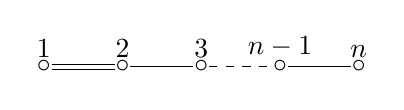
\begin{tikzpicture}[baseline=0]
			\node at (0,0) {$\circ$};
			\node[above] at (0, 0) {$1$};
			\draw[double equal sign distance] (0.1, 0) to (0.9,0);
			\node  at (1,0) {$\circ$};
			\node[above] at (1, 0) {$2$};
			\draw (1.1, 0) to (1.9,0);
			\node at (2,0) {$\circ$};		
			\node[above] at (2, 0) {$3$};
			\draw[dashed] (2.1, 0) to (2.9, 0);
			\node at (3, 0) {$\circ$}; 		
			\node[above] at (3, 0) {$n-1$};
			\node at (4, 0) {$\circ$};
			\node [above] at (4, 0) {$n$};
			\draw (3.1, 0) to (3.9, 0);
			\end{tikzpicture}
\]

We identify $W$ with the set of permutations $\s$ of $\{\pm 1, \pm 2, \ldots, \pm n\}$ with $\s(-i)=-\s(i)$ for all $i$. For $-n \le i, j \le n$, we define $$w[i, j]=\{-n \le k \le n; k \le i, w(k) \ge j\}.$$ We have the following explicit description of the Bruhat order. \remind{reference}

\begin{proposition}\label{B-i-j}
Let $x, y \in W$. Then $x \le y$ if and only if $\sharp x[i, j] \le \sharp y[i, j]$ for any $-n \le i, j \le n$.
\end{proposition}

The elliptic conjugacy classes of $W$ are parametrized by the partitions of $n$. Let $\underline \a=(a_1, a_2, \ldots, a_l)$ be a partition of $n$, i.e. $a_1 \ge a_2 \ge \cdots \ge a_l>0$ and $a_1+\cdots+a_l=n$. Let $O_{\underline \a}$ be the corresponding elliptic conjugacy class in $W$. This is the conjugacy class of $W$ consisting of permutations $w$ satisfying the following conditions:

\begin{enumerate}
	\item There exists a decomposition $\{1, 2, \ldots, n\}=I_1 \sqcup I_2 \sqcup \ldots \sqcup I_l$;
	
	\item $\sharp I_j=a_j$ for all $j$;
	
	\item The orbits of $w$ on $\{\pm 1, \ldots, \pm n\}$ are $I_j \sqcup -I_j$ for $1 \le j \le l$.
\end{enumerate}

We have the following useful inequalities for the elements in $O_{\underline \a}$.

\begin{proposition}\label{B-ineq}
	Let $w \in O_{\underline \a}$ and $0 \le m \le n$, we have $$\sharp w[n-m, n-m+1] \ge \min\{k; a_1+\cdots+a_k \ge m\}.$$
\end{proposition}

\begin{proof}
	Let $I_1, \ldots, I_l$ be the subsets of $\{1, \ldots, n\}$ satisfying the conditions (1)-(3) for $w$. Let $1 \le j \le l$ and $r=\max I_j$. Then $w^{\sharp I_j}(-r)=r$. Therefore if $r \ge n-m+1$, then there exists $s \in \BN$ such that $w^s(-r) \le n-m$ and $w^{s+1}(-r) \ge n-m+1$. In other words, $$w[n-m, n-m+1] \cap (I_j \sqcup -I_j) \neq \emptyset.$$ Therefore $$\sharp w[n-m, n-m+1] \ge \sharp\{j; \max I_j \ge n-m+1\}.$$
	
	Let $J=\{j; \max I_j \ge n-m+1\}$. Note that there are exactly $m$ elements in $I_1 \sqcup \ldots \sqcup I_l$ that are larger than or equal to $n-m+1$. We have $\sum_{j \in J} \sharp I_j \ge m$. As $\sharp I_k=a_k$ for all $k$ and $a_1 \ge \cdots \ge a_l$, we have $a_1+\cdots+a_{\sharp J} \ge \sum_{j \in J} \sharp I_j \ge m$. In other words, $\sharp J \ge \min\{k; a_1+\cdots+a_k \ge m\}$. The proposition is proved.
\end{proof}

Following \cite{He07}\footnote{Note that the convention for the labelling of the simple reflections here is opposite to the labelling used in \cite{He07} and the formulas belows are modified accordingly.}, for $1 \le a, b \le n$, we define $$s_{[a, b]}=\begin{cases} s_a s_{a+1} \cdots s_b, & \text{ if } a \le b; \\ 1, & \text{ otherwise}.\end{cases}$$

For any partition $\underline \a=(a_1, \ldots, a_l)$ of $n$, we define $$w_{\underline \a}=(s_{[2, n+1-a_1]} \i s_{[1, n]}) (s_{[2, n+1-a_1-a_2]} \i s_{[1, n-a_1]}) \cdots (s_{[1, a_l]}).$$ By \cite[\S 7]{He07}, $w_{\underline \a}$ is a minimal length element in $O_{\underline \a}$.

Now we prove the following result.

\begin{proposition}\label{B-main}
	Let $\underline \a, \underline \b$ be partitions of $n$. Then $O_{\underline \a} \preceq O_{\underline \b}$ if and only if $\underline \a \ge \underline \b$.
\end{proposition}

\begin{proof}
	If $\underline \a \ge \underline \b$, then $a_1 \ge b_1$, $a_1+a_2 \ge b_1+b_2$, $\ldots$. Thus \begin{gather*} s_{[2, n+1-a_1]} \i s_{[1, n]} \le s_{[2, n+1-b_1]} \i s_{[1, n]}, \\ s_{[2, n+1-a_1-a_2]} \i s_{[1, n-a_1]} \le s_{[2, n+1-b_1-b_2]} \i s_{[1, n-b_1]}, \\ \ldots. \end{gather*} So $w_{\underline \a} \le w_{\underline \b}$ and thus $O_{\underline \a} \preceq O_{\underline \b}$.
	
	On the other hand, if $O_{\underline \a} \preceq O_{\underline \b}$, then there exists $w \in O_{\underline \a}$ with $w \le w_{\underline \b}$. Let $m=b_1+\cdots+b_k$. By direct computation, we have $\sharp w_{\underline \b}[n-m, n-m+1]=k$. By Proposition \ref{B-i-j}, $\sharp w[n-m, n-m+1] \le k$. By Proposition \ref{B-ineq}, $k \ge \min\{k'; a_1+\cdots+a_{k'} \ge m\}$. In other words, $a_1+\cdots+a_k \ge m=b_1+\cdots+b_k$. Therefore $\underline \a \ge \underline \b$.
\end{proof}


\subsection{Type $D_n$ and ${}^2 D_n$} Let $W$ be the Weyl group of type $D_n$. We identify $W$ with the permutations $w$ of $\{\pm1, \dots, \pm n\}$ such that $w(-j) = -w(j)$ and $\sharp w[-1, 1]$ is even.
\begin{proposition} \label{D-i-j}
Let $x, y \in W$. If $x \leq y$, then $\sharp x[i, j] \le \sharp y[i, j]$ for any $-n \le i, j \le n$.
\end{proposition}

Let $\d$ be the permutation of $\{\pm1, \dots, \pm n\}$ such that $\d(1) = -1$ and $\d(k) = k$ for $2 \le k \le n$. The map $w \mapsto \d(w) := \d w \d\i$ is an outer involution of $W$. The map $W \to W\d: w \mapsto w\d$ induces a bijection from the set of $\d$-twisted conjugacy class of $W$ to the set of ordinary $W$-conjugacy classes of $W\d$.
\begin{proposition} \label{D-i-j-d}
Let $x, y \in W$. If $x \leq y$, then $\sharp \d x[i, j] \le \sharp \d y[i, j]$ for any $-n \le i, j \le n$.
\end{proposition}
\begin{proof}
Suppose otherwise. Then $\sharp \d x[a, b] > \sharp \d y[a, b]$ for some $-n \le a, b \le n$. For $z \in W$ one checks that $-1 \le \sharp z[i, j] - \sharp \d z[i, j] \le 1$, and moreover, $z[i, j] = \d z[i, j]$ (resp. $z[i, j] = z \d[i, j]$) if $j \neq 1$ (resp. $i \neq -1$).  As $x \leq y$ and $\d(x) \leq \d(y)$, we have $\sharp x[a, b] \le \sharp y[a, b]$ and $\sharp \d(x)[a, b] \le \sharp \d(y)[a, b]$ by Proposition \ref{D-i-j}. So we deduce that $a = -1$, $b = 1$ and $0 \le \sharp y[-1, 1] - \sharp x[-1, 1] \le 1$. Noticing that both $\sharp x[-1, 1]$ and $\sharp y[-1, 1]$ are even, we have $\sharp x[-1, 1] = \sharp y[-1, 1]$. Let $c = \min \{x(k), -1 \le k \le n, x(k) \ge 1\}$ and $d = \min \{y(k), -1 \le k \le n, y(k) \ge 1\}$. In particular, $d \ge c \ge 1$ as $\sharp x[-1, 1] = \sharp y[-1, 1]$.

If $d > 1$, then $\sharp y[-1, 1] = \sharp \d y[-1, 1] = \sharp \d x[-1, 1] - 1$, which means $c > 1$ and $x\i(-1) \le -1 < y\i(-1)$. If $d = 1$, then $c = 1$ and hence $\sharp \d x[-1, 1] = \sharp x[-1, 1] = \sharp \d y[-1, 1] + 1$, which also means $x\i(-1) \le -1 < y\i(-1)$. In either case, we have $\sharp x[-1, -1] = \sharp x[-1, 1] + 1 > \sharp y[-1, 1] = \sharp y[-1, -1]$, a contradiction.
\end{proof}


The elliptic conjugacy classes (resp. $\d$-twisted conjugacy classes) of $W$ are parameterized by the partitions of $n$ of even (resp. odd) lengths. Let $\underline \a=(a_1, a_2, \ldots, a_l)$ be a partition of $n$ of even length, i.e. $a_1 \ge a_2 \ge \cdots \ge a_l>0$, $a_1+\cdots+a_l=n$ and $l$ is even (resp. odd). Let $O_{\underline \a}$ (resp. ${}^2 O_{\underline \a}$) be the corresponding elliptic conjugacy class (resp. $\d$-twisted conjugacy classes) of $W$. This is the conjugacy class (resp. $\d$-twisted conjugacy classe) of $W$  consisting of permutations $w$ satisfying the following conditions:

\begin{enumerate}
	\item There exists a decomposition $\{1, 2, \ldots, n\}=I_1 \sqcup I_2 \sqcup \ldots \sqcup I_l$;
	
	\item $\sharp I_j=a_j$ for all $j$;
	
	\item The orbits of $w$ (resp. $w\d$) on $\{\pm 1, \ldots, \pm n\}$ are $I_j \sqcup -I_j$ for $1 \le j \le l$.
\end{enumerate}

\begin{proposition}\label{D-ineq}
For $0 \le m \le n$, we have \begin{align*}\sharp w[n-m, n-m+1] & \ge \min\{k; a_1+\cdots+a_k \ge m\} \text{ if } w \in O_{\underline \a}; \\ \sharp w\d[n-m, n-m+1] & \ge \min\{k; a_1+\cdots+a_k \ge m\} \text{ if } w \in {}^2 O_{\underline \a}. \end{align*}
\end{proposition}
\begin{proof}
It follows similarly as Proposition \ref{B-ineq}.
\end{proof}


\begin{proposition}\label{D-main}
Let $\underline \a, \underline \b$ be even (resp. odd) partitions of $n$. Then $O_{\underline \a} \preceq O_{\underline \b}$ (resp. ${}^2 O_{\underline \a} \preceq {}^2 O_{\underline \b}$) if and only if $\underline \a \ge \underline \b$.
\end{proposition}

\begin{proof}
We only consider the odd partition case. If $\underline \a \ge \underline \b$, then ${}^2 O_{\underline \a} \preceq {}^2 O_{\underline \b}$ follows similarly as in Proposition \ref{B-main} from the explicit constructions of minimal length elements $w_{\underline \a}$ and $w_{\underline \b}$ in ${}^2 O_{\underline \a}$ and ${}^2 O_{\underline \a}$ respectively.
	
On the other hand, if ${}^2 O_{\underline \a}\d \preceq {}^2 O_{\underline \b}$, then there exists $w \in {}^2 O_{\underline \a}$ with $w \leq w_{\underline \b}$. Let $m=b_1+\cdots+b_k$. By direct computation, we have $\sharp w_{\underline \b} \d[n-m, n-m+1]=k$. By Proposition \ref{D-i-j-d}, $\sharp w\d[n-m, n-m+1] \le k$. By Proposition \ref{D-ineq}, $k \ge \min\{k'; a_1+\cdots+a_{k'} \ge m\}$. In other words, $a_1+\cdots+a_k \ge m=b_1+\cdots+b_k$. Therefore $\underline \a \ge \underline \b$.
\end{proof}

\subsection{Type ${}^2 A_{n-1}$} Let $W=S_n$ be the group of permutations of $\{1, 2, \cdots, n\}$. For $1 \le i, j \le n$, we define $$w[i, j]=\{-n \le k \le n; k \le i, w(k) \ge j\}.$$ We have the following explicit description of the Bruhat order. \remind{reference}

\begin{proposition}\label{A-i-j}
Let $x, y \in W$. Then $x \le y$ if and only if $\sharp x[i, j] \le \sharp y[i, j]$ for any $1 \le i, j \le n$.
\end{proposition}

Let $\d=(1, n) (2, n-1) \cdots$ be the longest element of $W$. Then the conjugation action of $\d$ on $W$ induces a bijection on the set of simple reflections and is a length-preserving automorphism. The map $W \to W: w \mapsto w \d$ induces a bijection from the set of $\d$-twisted conjugacy class of $W$ to the set of ordinary conjugacy classes of $W$. Since $\d$ is the longest element of $W$, the map is order-reversing.

The $\d$-twisted elliptic conjugacy classes of $W$ are parametrized by the partitions of $n$ with odd parts. Let $\underline \a=(a_1, a_2, \ldots, a_l)$ be a partition of $n$ with odd parts, i.e. $a_1 \ge a_2 \ge \cdots \ge a_l>0$ are odd positive integers and $a_1+\cdots+a_l=n$. Let $O_{\underline \a}$ be the corresponding $\d$-twisted elliptic conjugacy class in $W$. This is the conjugacy class of $W$ consisting of permutations $w$ satisfying the following conditions:

\begin{enumerate}
	\item There exists a decomposition $\{1, 2, \ldots, n\}=I_1 \sqcup I_2 \sqcup \ldots \sqcup I_l$;
	
	\item $\sharp I_j=a_j$ for all $j$;
	
	\item The orbits of $w \d$ on $\{1, 2, \ldots, n\}$ are $I_j$ for $1 \le j \le l$.
\end{enumerate}

We have the following useful inequalities for the elements in $O_{\underline \a}$.

\begin{proposition}\label{A-ineq}
	Let $w \in O_{\underline \a}$ and $1 \le m \le n-1$, we have $$\sharp w\d[\lceil \frac{m}{2}\rceil, n-\lfloor \frac{m}{2} \rfloor+1]+\sharp w\d[n-\lfloor \frac{m}{2} \rfloor, \lceil \frac{m}{2}\rceil+1] \le n-\min\{k; a_1+\cdots+a_k \ge m\}.$$
\end{proposition}

\begin{proof} Let $I=w\d[\lceil \frac{m}{2}\rceil, n-\lfloor \frac{m}{2} \rfloor+1]$ and $I'=w\d[n-\lfloor \frac{m}{2} \rfloor, \lceil \frac{m}{2}\rceil+1]$. If $k \in I$, then $k \le \lceil \frac{m}{2}\rceil<\lceil \frac{m}{2}\rceil+1$ and thus $(w \d)\i (k) \notin I'$. In other words, $$I \cap (w \d) (I')=\emptyset.$$ Similarly,  $$I \cap (w \d) \i (I')=\emptyset.$$
	
In particular, for any $w\d$-orbit $I_j$, we have \[\tag{a}\sharp (I_j \cap I)+\sharp (I_j \cap I')=\sharp (I_j \cap I)+\sharp (I_j \cap (w \d)(I')) \le \sharp (I_j).\]

We claim that

(b) If $\sharp (I_j \cap I)+\sharp (I_j \cap I')= \sharp(I_j)$, then $I_j \subset \{\lceil \frac{m}{2}\rceil+1, \lceil \frac{m}{2}\rceil+2, \ldots, n-\lfloor \frac{m}{2} \rfloor\}$.

Note that $$\sharp(I_j \cap I)+\sharp(I_j \cap w \d(I'))=\sharp(I_j \cap I)+\sharp(I_j \cap (w \d) \i (I'))=\sharp(I_j).$$ Since $I \cap (w \d)(I')=I \cap (w \d) \i(I')=\emptyset$, we have $$(I_j \cap I) \sqcup (I_j \cap (w \d)(I'))=(I_j \cap I) \sqcup (I_j \cap (w \d) \i(I'))=I_j.$$ Thus $$(w \d) (I_j \cap I')=I_j \cap (w \d)(I')=I_j \cap (w \d) \i(I')=(w \d) \i(I_j \cap I').$$ In other words, $I_j \cap I'$ is a subset of $I_j$ that is stable under the action of $(w \d)^2$. Since the order of the action of $w \d$ on $I_j$ equals to $\sharp I_j$, which is an odd integer. Hence $I_j \cap I'$ is a $w \d$-stable subset of $I_j$. As $w \d$ acts transitively on $I_j$, we have $I_j \cap I'=\emptyset$ or $I_j$. Hence $I_j \subset I$ or $I_j \subset I'$. However, as $\lceil \frac{m}{2} \rceil<n-\lfloor \frac{m}{2} \rfloor+1$, if $k \in I$, then $(w \d)(k) \notin I$. Thus $I_j \subset I'$. In other words, for any $k \in I_j$, $k \ge \lceil \frac{m}{2} \rceil+1$ and $k \le n-\lfloor \frac{m}{2} \rfloor$.

(b) is proved.

Let $J=\{j; I_j \not\subset \{\lceil \frac{m}{2}\rceil+1, \lceil \frac{m}{2}\rceil+2, \ldots, n-\lfloor \frac{m}{2} \rfloor\}\}$. By (a) and (b), we have that $$\sharp J+\sharp J'=\sum_j (\sharp (I_j \cap J)+\sharp(I_j \cap J')) \le \sum_j \sharp(I_j)-\sharp J=n-\sharp J.$$ Note that there are exactly $m$ elements outside $\{\lceil \frac{m}{2}\rceil+1, \lceil \frac{m}{2}\rceil+2, \ldots, n-\lfloor \frac{m}{2} \rfloor\}$. We have $\sum_{j \in J} \sharp I_j \ge m$. As $\sharp I_k=a_k$ for all $k$ and $a_1 \ge \cdots \ge a_l$, we have $a_1+\cdots+a_{\sharp J} \ge \sum_{j \in J} \sharp I_j \ge m$. In other words, $\sharp J \ge \min\{k; a_1+\cdots+a_k \ge m\}$. The proposition is proved.
\end{proof}

Now we prove the following result.

\begin{proposition}
	Let $\underline \a, \underline \b$ be partitions of $n$ with odd parts. Then $O_{\underline \a} \preceq O_{\underline \b}$ if and only if $\underline \a \ge \underline \b$.
\end{proposition}

\begin{proof}
	The strategy is similar to the proof of Proposition \ref{B-main}.
	
	We use the explicit minimal length elements $w_{\underline \a}$ of $O_{\underline \a}$ constructed in \cite[Lemma 7.13]{He07}.
	If $\underline \a \ge \underline \b$, then $a_1 \ge b_1$, $a_1+a_2 \ge b_1+b_2$, $\ldots$. By the explicit formula, $w_{\underline \a} \le w_{\underline \b}$ and thus $O_{\underline \a} \preceq O_{\underline \b}$.
	
	On the other hand, if $O_{\underline \a} \preceq O_{\underline \b}$, then there exists $w \in O_{\underline \a}$ with $w \le w_{\underline \b}$. Hence $w \d \ge w_{\underline \b} \d$. Let $m=b_1+\cdots+b_k$. By direct computation, we have $$\sharp w_{\underline \b} \d[\lceil \frac{m}{2}\rceil, n-\lfloor \frac{m}{2} \rfloor+1]+\sharp w_{\underline \b} \d[n-\lfloor \frac{m}{2} \rfloor, \lceil \frac{m}{2}\rceil+1]=n-k.$$
	
	By Proposition \ref{A-i-j}, $$\sharp w \d[\lceil \frac{m}{2}\rceil, n-\lfloor \frac{m}{2} \rfloor+1]+\sharp w \d[n-\lfloor \frac{m}{2} \rfloor, \lceil \frac{m}{2}\rceil+1]\ge n-k.$$ By Proposition \ref{A-ineq}, $k \ge \min\{k'; a_1+\cdots+a_{k'} \ge m\}$. In other words, $a_1+\cdots+a_k \ge m=b_1+\cdots+b_k$. Therefore $\underline \a \ge \underline \b$.
\end{proof}

\begin{thebibliography}{AAAA99}
\bibitem[DHM13]{DHM}
O. Dudas, X. He and J. Michel, \emph{Private communication}, 2013.

\bibitem[DL76]{DL}
P. Deligne and G. Lusztig, \emph{Representations of reductive groups over finite fields}, Ann. of Math. (2) 103 (1976), no. 1, 103--161.

\bibitem[DM15]{DM}
O. Dudas and G. Malle, \emph{Decomposition matrices for low-rank unitary groups}, Proc. Lond. Math. Soc. (3) 110 (2015), no. 6, 1517--1557.

\bibitem[JO00]{JO}
A. J. de Jong and F. Oort, \emph{Purity of the stratification by Newton polygons}, J. Amer. Math. Soc. 13 (2000), 209--241.

\bibitem[Lu11]{L1}
G. Lusztig, \emph{From conjugacy classes in the Weyl group to unipotent classes}, Represent. Theory 15 (2011), 494--530.

\bibitem[Lu12]{L3}
G. Lusztig, \emph{From conjugacy classes in the Weyl group to unipotent classes, III}, Represent. Theory 16 (2012), 450--488.

\bibitem[Ha15]{Ha}
P. Hamacher, \emph{The geometry of Newton strata in the reduction modulo p of Shimura varieties of PEL type}, Duke Math. J. 164 (2015), no. 15, 2809--2895.

\bibitem[HV11]{HV}
U. Hartl and E. Viehmann, \emph{The Newton stratification on deformations of local G-shtukas}, J. Reine Angew. Math. 656 (2011), 87--129.

\bibitem[He07]{He07}
X. He, {\em Minimal length elements in some double cosets of Coxeter groups},  Adv. Math. 215 (2007), 469--503.

\bibitem[He14]{He-Ann}
X. He, \emph{Geometric and homological properties of affine Deligne-Lusztig varieties}, Ann. of Math. (2) 179 (2014), 367--404.

\bibitem[He16a]{He-CDM}
X. He, \emph{Hecke algebras and $p$-adic groups}, Current developments in mathematics 2015, 73--135, Int. Press, Somerville, MA, 2016.

\bibitem[He16b]{He-KR}
X. He, \emph{Kottwitz-Rapoport conjecture on unions of affine Deligne-Lusztig varieties},  Ann. Sci. \`Ecole Norm. Sup. 49 (2016), 1125--1141.

\bibitem[HN14]{HN2}
X. He and S. Nie, \emph{Minimal length elements of extended affine Weyl group}, Compos. Math. 150 (2014), 1903--1927.

\bibitem[Sp82]{Spa}
N. Spaltenstein, \emph{Classes unipotents et sous-groupes de Borel}, Lecture Notes in Math. 946, Springer, 1982.

\bibitem[Vi13]{Vi}
E. Viehmann, \emph{Newton strata in the loop group of a reductive group}, Amer. J. Math. 135 (2013), no. 2, 499--518.

\bibitem[Wa63]{Wall}
G. E. Wall, \emph{On the conjugacy classes in the unitary, symplectic and orthogonal groups},  J. Austral. Math. Soc., 3 (1963), 1--63.

\end{thebibliography}


\end{document}
